\documentclass[11pt,          % font size: 11pt or 12pt
               ms,            % degree:    ms or phd
               onehalfspacing % spacing: onehalfspacing or doublespacing
               ]{ncsuthesis}

%%----------------------------------------------------------------------------%%
%%------------------------------ Import Packages -----------------------------%%
%%----------------------------------------------------------------------------%%

\usepackage{booktabs}  % professionally typeset tables
\usepackage{amsmath}%,amssymb,amsfonts}
\usepackage{textcomp}  % better copyright sign, among other things
\usepackage{lipsum}    % filler text
\usepackage{subfig}    % composite figures

%%%%%%%%%%%%%%%%%%%%%%%%%%%%%%%%%%%%%%%%%%
%%%%%%%%%%% Hack for alphanumeric bibliography
%%%%%%%%%%%%%%%%%%%%%%%%%%%%%%%%%%%%%%%%%%5
\RequirePackage[
			style=alphabetic,%numeric-comp,%authoryear-comp,%
			sorting=nyt,%ynt					
			hyperref=true, %	
			giveninits=true,%
			%backend=bibtex,
			natbib=true,
			url=false,
			isbn=false,
			maxnames=2, %for et al to be used
			maxalphanames=1, %to avoid printing a + for every et al in abbreviation
			doi=false]{biblatex}		
			
%needed to do et al after two names
%http://tex.stackexchange.com/questions/44048/use-et-al-in-biblatex-custom-style
\renewcommand*{\finalnamedelim}{\addspace\&\space}

%Simplify abbreviation (the default uses either one or two authors and it 
%indicates et al with a +) The following five lines make it so that only the 
%first author is used in the abbreviation
%http://tex.stackexchange.com/questions/27956/label-only-from-first-author
\renewcommand*{\labelalphaothers}{}
    \renewcommand*{\intitlepunct}{}
    \DefineBibliographyStrings{german}{in={}}
    \DefineBibliographyStrings{english}{in={}}
    \DeclareNameAlias{sortname}{last-first}
    \DeclareNameAlias{default}{last-first}
	
\DeclareFieldFormat[article,periodical]{volume}{\mkbibbold{#1}}
\makeatletter

\newrobustcmd*{\parentexttrack}[1]{%
  \begingroup
  \blx@blxinit
  \blx@setsfcodes
  \blx@bibopenparen#1\blx@bibcloseparen
  \endgroup}

\AtEveryCite{%
  \let\parentext=\parentexttrack%
  \let\bibopenparen=\bibopenbracket%
  \let\bibcloseparen=\bibclosebracket}

\makeatother
\renewcommand{\cite}[1]{\parencite{#1}}

\renewbibmacro{in:}{%
  \ifentrytype{article}{}{%
  \printtext{\bibstring{in}\intitlepunct}}}
  
\AtEveryBibitem{\clearfield{month}}

\AtEveryBibitem{\clearfield{language}}

%%%%%%%%%%%%%%%%%%%%%%%%%%%%%%%%%%%%%%%%%%%%%

\addbibresource{WilliamDawn-thesis.bib}
 \defbibheading{myheading}[BIBLIOGRAPHY]{
 \chapter*{#1}
 \markboth{#1}{#1}}

%amssymb and amsfonts cannot be used in conjunction with mdput
%\usepackage{amsmath,amssymb,amsfonts}
\usepackage{dcolumn}% Align table columns on decimal point
\usepackage{bm}% bold math
%\usepackage{hyperref}% add hypertext capabilities
%\usepackage{hypernat}% make hyperref and natbib work together
\usepackage{cancel}
\usepackage{verbatim}% multiline commenting
\usepackage{ifthen}
\usepackage{url}
\usepackage{sectsty}
\usepackage{balance} 
%\usepackage{caption}
\usepackage{graphicx} %eps figures can be used instead
\usepackage{lastpage}
\usepackage[format=plain,
  justification=RaggedRight,
  singlelinecheck=false,
  font=small,labelfont=bf,
  labelsep=space]{caption} 
\usepackage{fancyhdr}
\pagestyle{fancy}

%http://tex.stackexchange.com/questions/100817/error-when-using-bc-from-abbrevs-in-caption
%Getting BC
\usepackage{abbrevs}
\usepackage{etoolbox}
\robustify{\DateMark} % after having loaded abbrevs

%Needed to solve bug from citation Hydrodynamics in 21/2 dimensions
\usepackage{units}
%see http://www.latex-community.org/viewtopic.php?f=5&t=989

\usepackage[sharp]{easylist} %used for brainstorming purposes 
% used for \Asterisk for convolution %conflicts with \widering
%\usepackage{mathabx}

%compile on single pass
%\usepackage[backend=biber,...]{biblatex}

%%%%%%%%%%%%
%%% Hack to make chapters start on odd pages
% http://tex.stackexchange.com/questions/73591/how-to-have-a-blank-even-page-before-every-chapter
%%%%%%%%%%%%
%\newcommand{\ensureoddstart}{\checkoddpage\ifoddpage\else\newpage\mbox{}\fi}
%\newcommand{\ensureoddstart}{}

%%%Fancy tables
%http://tex.stackexchange.com/questions/94032/fancy-tables-in-latex
\usepackage[table]{xcolor}
\usepackage{array,booktabs}
\usepackage{colortbl}
\newcolumntype{L}{@{}>{\kern\tabcolsep}l<{\kern\tabcolsep}}

%%%%%%%%%%
%%%%% Hack to allow more levels in outline
%%%%%%%%%%
%\setcounter{secnumdepth}{5}
%\setcounter{tocdepth}{5} %may violate ETD
%Usage http://pleasemakeanote.blogspot.com/2010/06/how-to-activate-subsubsubsection-in.html
%\section{} % level 1
%\subsection{} % level 2
%\subsubsection{} % level 3
%\paragraph{} % level 4 - equivalent to subsubsubsection
%\subparagraph{} % level 5

%http://tex.stackexchange.com/questions/60209/how-to-add-an-extra-level-of-sections-with-headings-below-subsubsection
\usepackage{titlesec}

\setcounter{secnumdepth}{4}

\titleformat{\paragraph}
{\normalfont\normalsize\bfseries}{\theparagraph}{1em}{}
\titlespacing*{\paragraph}
{0pt}{3.25ex plus 1ex minus .2ex}{1.5ex plus .2ex}

%%%%%%%%%%%%%%%%%%%%%%%%%%
%%%% Hack for containing figures within sections
%%%%%%%%%%%%%%%%%%%%%%%%%%%%
%http://ctan.org/pkg/placeins
\usepackage{placeins}
%Defines a \FloatBarrier com�mand, beyond which floats may not pass; useful,
%for example, to ensure all floats for a section appear be�fore the next 
%\section command.

%%%Hack for centering all figures
%\makeatletter
%\g@addto@macro\@floatboxreset\centering
%\makeatother

%%----------------------------------------------------------------------------%%
%%---------------------------- Formatting Options ----------------------------%%
%%----------------------------------------------------------------------------%%
%%

%% -------------------------------------------------------------------------- %%
%% Disposition format -- any titles, headings, section titles
%%  These formatting commands affect all headings, titles, headings,
%%  so sizing commands should not be used here.
%%  Formatting options to consider are
%%     +  \sffamily - sans serif fonts.  Dispositions are often typeset in
%%                    sans serif, so this is a good option. 
%%     +  \rmfamily - serif fonts
%%     +  \bfseries - bold face
%\dispositionformat{\sffamily\bfseries}   % bold and sans serif
\dispositionformat{\bfseries}            % bold and serif

%% -------------------------------------------------------------------------- %%
%% Formatting for centered headings - Abstract, Dedication, etc. headings
%%  This is where one might put a sizing command.
%%  \MakeUppercase can be used to typeset all headings in uppercase.
\headingformat{\large\MakeUppercase}   % All letters uppercase
%\headingformat{\large}                % Not all uppercase
%\headingformat{\Large\scshape}        % Small Caps, used with serif fonts.

%% Typographers recommend using a normal inter-word space after
%% sentences. TeX's default is to add an wider space, but \frenchspacing
%% gives a normal spacing. Comment out the following line if you prefer
%% wider spaces between sentences.
\frenchspacing

%% -------------------------------------------------------------------------- %%
%%  Optional packages
%%    A number of compatible packages to improve the look and feel of
%%    your document are available in the file optional.tex 
%%    (For example, hyperlinks, fancy chapter headings, and fonts)
%% To use these options, uncomment the next line and see optional.tex
%%  Optional Packages to consider.   These packages are compatible with
%%    ncsuthesis.  

%% -------------------------------------------------------------------------- %%
%% Fancy chapter headings
%%  available options: Sonny, Lenny, Glenn, Conny, Rejne, Bjarne
% \usepackage[Conny]{fncychap}
\usepackage[Rejne]{fncychap}

%%----------------------------------------------------------------------------%%
%% Hyperref package creates PDF metadata and hyperlinks in Table of Contents
%%  and citations.  Based on feedback from the NCSU thesis editor, 
%%  the links are not visually distinct from normal text (i.e. no change
%%  in color or extra boxes).
\usepackage[
  pdfauthor={William C. Dawn},
  pdftitle={SFR with FEM Multiphysics},
  pdfcreator={pdftex},
  pdfsubject={NC State ETD Thesis},
  pdfkeywords={nuclear, sodium, fast, reactor, nuclear reactor, 
    finite element, multiphysics},
  colorlinks=true,
  linkcolor=black,
  citecolor=black,
  filecolor=black,
  urlcolor=black,
]{hyperref}


%% -------------------------------------------------------------------------- %%
%% Microtype - If you use pdfTeX to compile your thesis, you can use
%%              the microtype package to access advanced typographic
%%              features.  By default, using the microtype package enables
%%              character protrusion (placing glyphs a hair past the right 
%%              margin to make a visually straighter edge)
%%              and font expansion (adjusting font width slightly to get 
%%              more favorable justification).
%%              Using microtype should decrease the number of lines
%%              ending in hyphens.
\usepackage{microtype}


%%----------------------------------------------------------------------------%%
%% Fonts 

%% ETD guidelines don't specify the font.  You can enable the fonts
%%  by uncommenting the appropriate lines.  Using the default Computer 
%%  Modern fonts is *not* required.  A few common choices are below.
%%  See http://www.tug.dk/FontCatalogue/ for more options.

%% Serif Fonts -------------------------------------------------
%%  The four serif fonts listed here (Utopia, Palatino, Kerkis,
%%  and Times) all have math support.


%% Utopia
%\usepackage[T1]{fontenc}
%\usepackage[adobe-utopia]{mathdesign}

%% Palatino
%\usepackage[T1]{fontenc}
%\usepackage[sc]{mathpazo}
%\linespread{1.05}

%% Kerkis
%\usepackage[T1]{fontenc}
%\usepackage{kmath,kerkis}

%% Times
\usepackage[T1]{fontenc}
\usepackage{mathptmx}
\usepackage{amsmath}


%% Sans serif fonts -------------------------

% this will work with math and text
%\renewcommand{\familydefault}{\sfdefault}
%\usepackage[scaled]{helvet}  % Helvetica
%\usepackage[cm]{sfmath}

%\usepackage[scaled]{berasans} % Bera Sans

%solve bug from fancyhdr in optional
%http://nw360.blogspot.com/2006/11/latex-headheight-is-too-small.html
\setlength{\headheight}{14pt}

%%----------------------------------------------------------------------------%%
%%---------------------------- Content Options -------------------------------%%
%%----------------------------------------------------------------------------%%
%% Size of committee: 3, 4, 5, or 6 -- this number includes the chair
\committeesize{4}

%% Members of committee
%%  Each of the following member commands takes an optional argument
%%   to specify their role on the committee.
%%  For co-chairs, use the commands:
%%      \cochairI{Doug Dodd}
%%      \cochairII{Chris Cox}
%%
\cochairI{Scott P. Palmtag}
\cochairII{David J. Kropaczek}
\memberI{Joseph M. Doster}
\memberII{Zhilin Li}

%% Student writing thesis, \student{First Middle}{Last}
\student{William C.}{Dawn}

%% Degree program
\program{Nuclear Engineering}

%% Thesis Title
%%  Keep in mind, according to ETD guidelines:
%%    +  Capitalize first letter of important words.
%%    +  Use inverted pyramid shape if title spans more than one line.
%%
%%  Note: To break the title onto multiple lines, use \break instead of \\.
%\thesistitle{A North Carolina State University Sample \LaTeX{} Thesis \break 
%with a Title So Long it Needs a Line Break}
\thesistitle{Sodium Cooled Fast Reactor Simulations with the Finite Element
Method}

%% Degree year.  Necessary if your degree year doesn't equal the current year.
%\degreeyear{1995}

%%----------------------------------------------------------------------------%%
%%---------------------------- Personal Macros -------------------------------%%
%%----------------------------------------------------------------------------%%

%% A central location to add your favorite macros.

%% A few examples to get you started.
\newcommand{\uv}[1]{\ensuremath{\mathbf{\hat{#1}}}}
\newcommand{\bo}{\ensuremath{\mathbf{\Omega}}}
\newcommand{\del}{\nabla}
\renewcommand{\exp}[1]{e^{#1}}
\newcommand{\Conv}{\mathop{\scalebox{1.5}{\raisebox{-0.2ex}{$\ast$}}}}%

% reference macros
\newcommand{\eref}[1]{Eq.~\ref{#1}}
\newcommand{\fref}[1]{Fig.~\ref{#1}}
\newcommand{\tref}[1]{Table~\ref{#1}}

\usepackage{color}
\newcommand{\NEW}[1]{#1}
\newcommand{\COMMENT}[1]{\textcolor{green}{#1}}

\newcommand{\NOTER}[1]{\textcolor{orange}{#1}}
\newcommand{\NOTEC}[1]{\textcolor{blue}{#1}}
\newcommand{\NOTEK}[1]{\textcolor{magenta}{#1}}

\newcommand{\mum}{\ensuremath{{\mu}\text{m}}}

%This makes it so that you can add short paths in your .tex by including the
%folders where you store your images in the search path
\graphicspath{{./Chapter-1/figs/}{./Chapter-2/figs/}{./Chapter-3/figs/}}%{./Chapter-4/figs/}{./Chapter-5/figs/}{./Chapter-6/figs/}}

%%---------------------------------------------------------------------------%%
\usepackage{calc}
%% Capital letter height
\newlength{\chaptercapitalheight}
\settoheight{\chaptercapitalheight}{D}
\newlength{\chapterfootskip}
\setlength{\chapterfootskip}{\chaptercapitalheight}
\addtolength{\chapterfootskip}{2\baselineskip}
% A little extra space to ensure there are 2 full double spaced lines
\addtolength{\chapterfootskip}{0.5ex}
%\def\chapterfootskipnum{\chapterfootskip}
\renewcommand{\listfigurename}{LIST OF FIGURES}
\renewcommand{\listtablename}{LIST OF TABLES}
\renewcommand{\bibname}{BIBLIOGRAPHY}

%\renewcommand{\cfttoctitlefont}{\centering\ncsu@headingformat}

%http://tex.stackexchange.com/questions/47184/height-of-figure-caption-textheight
\newlength\graphht
\newcommand\calculategraphicstargetheight[1]{%
     \setlength\graphht{\textheight 
                       -\parskip
                       -\abovecaptionskip -\belowcaptionskip
                       -(12pt * #1) % assuming baselineskip of 12pt in caption
                       -\chapterfootskip
                       }}
%\usepackage{titlesec}

%landscape support in fancyhdr from 
%http://tex.stackexchange.com/questions/9071/how-to-translate-and-rotate-the-heading-of-landscaped-pages
\usepackage{pdflscape}
\usepackage{tikz}
\fancypagestyle{lscapedplain}{%
  \fancyhf{}
  \fancyfoot{%
    \tikz[remember picture,overlay]
      \node[outer sep=1cm,above,rotate=90] at (current page.east) {\thepage};}
\renewcommand{\headrulewidth}{0pt} 
\renewcommand{\footrulewidth}{0pt}
}

\begin{document}
\pagestyle{plain}
%%---------------------------------------------------------------------------%%
\frontmatter
%% ------------------------------ Abstract ---------------------------------- %%
\begin{abstract}
  Renewed interest in advanced nuclear power reactors such as the Versatile Test 
  Reactor (VTR) at Idaho National Laboratory (INL) has encouraged enhanced 
  modeling of Sodium Cooled Fast Reactors (SFRs). Since their inception in the 
  early days of nuclear engineering with reactors such as at the Experimental 
  Breeder Reactor and Fermi 1, many new modeling techniques have been developed.
  This work seeks to introduce cutting-edge methods to the simulation of SFRs.

  In this work, the multigroup neutron diffusion equation is solved via the
  Finite Element Method (FEM). This method allows for the use of unstructured
  and general meshes. By using an unstructured mesh, physical phenomena such as
  thermal expansion can be modeled and used to perturb the mesh. Additionally,
  the FEM will allow for simplified mesh refinements by means of both geometric
  refinement and the use of higher order methods without recreating the mesh.
  The multigroup neutron diffusion equation can be solved for two-dimensional
  problems using triangles or three-dimensional problems using pentahedra, also
  known as wedges. 

  Thermal feedback effects within a SFR are also modeled in this work. A
  simplified thermal hydraulic model is used, modeling both axial heat 
  convection and radial heat conduction. Resulting temperatures are used to 
  calculate on-the-fly neutron cross-sections to capture the effects of Doppler
  feedback. Additionally, a thermal expansion model is used to simulate the 
  thermal expansion of fuel and structural components within the reactor. These 
  effects have been proven to significantly impact reactor behavior in 
  experiments such as those performed at Experimental Breeder Reactor II 
  (EBR-II).

  Using these models, a typical SFR is simulated at operating conditions. The 
  models as implemented demonstrate expected reactor behavior for an SFR and can
  be used to visualize the inherent safety features and feedback effects of such 
  a nuclear reactor.
  
\end{abstract}

%% ---------------------------- Copyright page ------------------------------ %%
\makecopyrightpage

%% -------------------------------- Title page ------------------------------ %%
\maketitlepage

%% -------------------------------- Dedication ------------------------------ %%
\begin{dedication}
  \centering To the future of clean electricity and natural beauty.
\end{dedication}

%% -------------------------------- Biography ------------------------------- %%
\begin{biography}
  William C. Dawn was born and raised in Stafford, Virginia. He attended public
  schools there for his primary education, participating in the Commonwealth
  Governor's School for High School. William earned a B.S. degree in Nuclear
  Eneingeering from North Carolina State University (NC State) in May 2017. 
  After his Master's degree, William will remain at NC State to pursue a Ph.D.
  degree in Nuclear Engineering. 

  William is a fellow of the Integrated University Program (IUP) facilitated by
  DOE-NE. During his undergraduate and graduate careers, he has had the
  opportunity to work with GE-Hitachi Nuclear Energy LLC. and Oak Ridge National
  Laboratory (ORNL). William has also made contributions to the Consortium for
  Advanced Simulation of LWRs (CASL).
\end{biography}

%% ----------------------------- Acknowledgements --------------------------- %%
\begin{acknowledgements}
  This work would not have been possible without the help of friends and family.
  I would like to thank my Mom and Dad, Suzanne and Bill Dawn, for their
  patience, their listening, and their advice. Their support has helped to make
  this work a reality.

  I would also like to thank my advisor, Dr. Scott Palmtag. We have both learned
  tremendously during this process. His consistency and desire to know more have
  kept me busy these last few months and I am grateful.
\end{acknowledgements}

%% ----------------------------- Disclaimer --------------------------- %%
\clearpage
\vspace*{\fill}
\begin{center}
  \mbox{\parbox{5in}{
  This material is based upon work supported under an Integrated
  University Program Graduate Fellowship. Any opinions, findings, conclusions,
  or recommendations expressed in this publication are those of the author and
  do not necessarily reflect the views of the Department of Energy Office of
  Nuclear Energy.
  }}
\end{center}
\vspace*{\fill}
\clearpage

\thesistableofcontents

\thesislistoftables

\thesislistoffigures

%%---------------------------------------------------------------------------%%
\mainmatter

\pagestyle{plain}
\newgeometry{margin=1in,lmargin=1.25in,footskip=\chapterfootskip, includehead, 
  includefoot}
\chapter{INTRODUCTION}
\label{chap-one}
Let's start with a few paragraph basics, here is how to make \textbf{bold}, 
and \textit{italics}, and \emph{emphasized}.  Let's say you need to cite 
something in your references, simply type \verb^\cite{key}^, which produces
\cite{einstein1935particle}.  
Some other references are \cite{golub1996matrix} and 
\cite{larsen1974asymptotic}.
Some \LaTeX{} compilers 
require a second compilation for citations and references 
to be sorted and matched properly in the resulting document.  

Here is a quotation:
\begin{quotation}
Alice, Bob and Carol are boring.  Who would even want to know their secret?
\end{quotation}

Let's say we need to make a list, try this on for size
\begin{enumerate}
  \item NCSU is great
  \item I like NCSU
  \item I really hope I can find a job when I graduate!
\end{enumerate} 

\section{Math enviroments}
\subsection{Equations}

There are many different ways to write equations, for example we could put 
$a^2 + b^2 = c^2$ directly into a sentence.  Or we could use the equation 
enviroment and do 
%
\begin{equation}
  a^2+b^2=c^2.
  \label{eq:one}
\end{equation} 
And from here we can later reference it by simply doing typing 
\verb^\ref{label}^, which gives \ref{eq:one}.  However, defining and using
equation and figure reference macros will ensure that the equation
references are consistent, instead of having Eq.~(1), Equation 3, Eqn 4
scattered through the thesis.  This template file defines \verb^\eref^
and \verb^\fref^ for this purpose. You can modify the macros to your liking
in the \texttt{YourName-thesis.tex} file.
For example, the command \verb^\eref{label}^ gives \eref{eq:one}.


If you don't need to reference an equation you may simply do this 
\[
  a^2 + b^2 = c^2.
\]

For Greek letters you must go to the math enviroments, for example 
$\alpha$, $\beta$, and $\gamma$.  Let's look at equations that cover 
multiple lines, none of these equations may be true or mean anything, but so 
that the reader can get some ideas.  In addition I will use some other useful 
notations like subscripts, superscripts, fractions, etc.  One important item 
of note is that one uses the ``ampersand" symbol to line up equations 
(also look at how I used quotations).
%
\begin{eqnarray}
\gamma_1 & = & \alpha^{\beta} + \psi_0 \frac{\psi_1}{\psi_2+\psi_3} \label{eq.two} \\
& = & \beta_1 + \beta_2 + \ldots + \beta_k \nonumber\\
& \rightarrow & E(\gamma_2) 
\end{eqnarray}

Alternatively, one can specify a slightly different enviroment if none of 
the equations need to be numbered.  Remember that if you are planning on 
referring to them later on, you must use a ``label" statement.
%
\begin{eqnarray*}
\gamma_1 & = & n^{-1/2} \displaystyle \sum_{i=1}^n \left[h(X_i,\beta_0)-E\{h(X_i,\beta_0)\}\right]\\
& \rightarrow & \hat q \pm \frac{\partial \gamma_2}{\partial \beta}. 
\end{eqnarray*}  
Lastly there may be times in which you want to use a non-italicized word 
your formula, such as an indicator function that may look like this 
$\mbox{I}\{\mu_i(1,\beta)>\mu_i(0,\beta)\}$ , if so just use the 
``mbox" statement.


You could use a multiline equation for long equations.  The environment
is \texttt{multline}.  Insert \verb^\\^ for line breaks.

\begin{multline*}
\bo \cdot \vec{\nabla} \psi(\vec{r},\bo ,E) + \Sigma_t(\vec{r},E)\psi(\vec{r},\bo ,E) = \\
  \int_{4\pi} d\bo' \int_0^{\infty} dE' \, \Sigma_s(\vec{r},\bo'\to\bo,E'\to E)\psi(\vec{r},\bo',E') + Q(\vec{r},\bo ,E),
\end{multline*}


we operate with $\displaystyle\int_{0}^{\infty}\left(\,\cdot\,\right) dE$
to obtain
\begin{multline*}
  \bo \cdot \vec{\nabla} \tilde{\psi}(\vec{r},\bo)
  + \Sigma_t(\vec{r})\tilde{\psi}(\vec{r},\bo) = \\
  \int_{4\pi} d\bo' \int_0^{\infty} dE' \, \psi(\vec{r},\bo',E')
  \left [ \int_{0}^{\infty} dE \, \Sigma_s(\vec{r},\bo'\to\bo,E'\to E)
  \right ] + \tilde{Q}(\vec{r},\bo),
\end{multline*}


\chapter{TABLES, FIGURES AND MATRICES}
\label{chap-two}
In Chapter \ref{chap-one} we did some typesetting and equations; now let's 
look at tables, figures, and matrices.

\section{Tables}
Table \ref{tab:one} is about as simple as they come, to put a formula in a 
table just use the same methods as putting a formula in a paragraph.  
Table \ref{tab:two} is a similar table in landscape on a seperate page.  
%
\begin{table}
\caption{Table Example}
\label{tab:one}
\begin{center}
\begin{tabular}{lccl}
\toprule
Treatment & No Death & Death & Total\\
\midrule
Therapy A & 1295 & 72 & 1367\\
Therapy B 	& 2294 & 195 & 2489\\
\midrule
Total & 3589 & 267 & 3856\\
\bottomrule
\end{tabular}
\end{center}
\end{table}

\paragraph{Filler Text} \lipsum[1-2]

\newgeometry{margin=1in,lmargin=1.25in,footskip=\chapterfootskip, includehead, includefoot}
\thispagestyle{lscapedplain}
\begin{landscape}
\begin{table}
\caption{Landscape Table Example}
\label{tab:two}
\begin{center}
\begin{tabular}{lcccccccccl}
\toprule
Patient & A & B & C & D & E & F & G & H &I & Total \\
\midrule
John & 1 & 2 & 3 & 4 & 5 & 6 & 7 & 8 & 9 & 45 \\
Amy & 1 & 2 & 3 & 4 & 5 & 6 & 7 & 8 & 9 & 45 \\
Jim & 1 & 2 & 3 & 4 & 5 & 6 & 7 & 8 & 9 & 45 \\
Jason & 1 & 2 & 3 & 4 & 5 & 6 & 7 & 8 & 9 & 45 \\
Sandy & 1 & 2 & 3 & 4 & 5 & 6 & 7 & 8 & 9 & 45 \\
Icem & 1 & 2 & 3 & 4 & 5 & 6 & 7 & 8 & 9 & 45 \\
\midrule
Total & 6 & 12 & 18 & 24 & 30 & 36 & 42 & 48 & 54 & 270\\
\bottomrule
\end{tabular}
\end{center}
\end{table}
\end{landscape}
\restoregeometry
\pagestyle{plain}
\thispagestyle{plain}
\newgeometry{margin=1in,lmargin=1.25in,footskip=\chapterfootskip, includehead, includefoot}


\section{Figures}

The easiest way to insert a picture is to have that picture in pdf format.  
\fref{fig:hist1} and \fref{fig:hist2} are two figures typeset normally.
ETD guidelines allow the use of landscape pages in the electronic 
submission.  To rotate a page, do NOT use the \texttt{lscape} environment. 
Instead, use the \texttt{pdflscape} package, for compatibility with PDFlatex.
Please note, if you are preparing a document for binding, consider
giving the \texttt{hardcopy} option in the \verb|\documentclass|
declaration.  This will place the page number at the normal location,
which is where it should be for printing and binding.

\begin{figure}[hbtp]
\centering
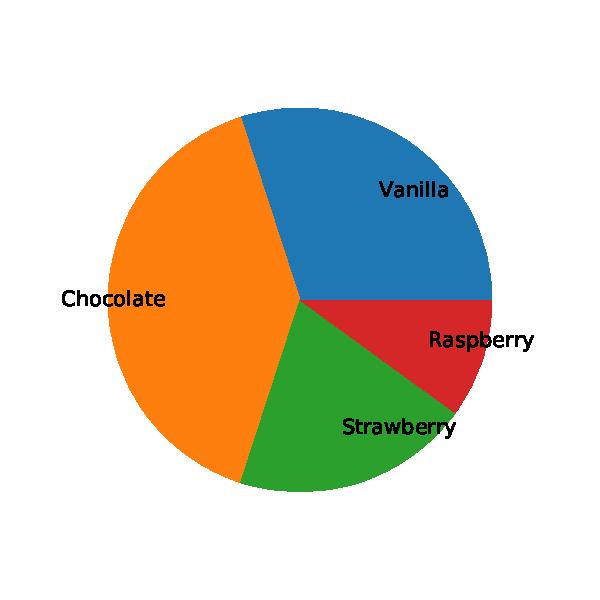
\includegraphics[width=0.6\textwidth]{Chapter-2/figs/pie}
\caption{Here is a sample figure}
\label{fig:hist1}
\end{figure}

For an example of a figure with a really long caption, see Fig.~\ref{fig:longcap}
\begin{figure}[hbtp]
\centering
\calculategraphicstargetheight{11}
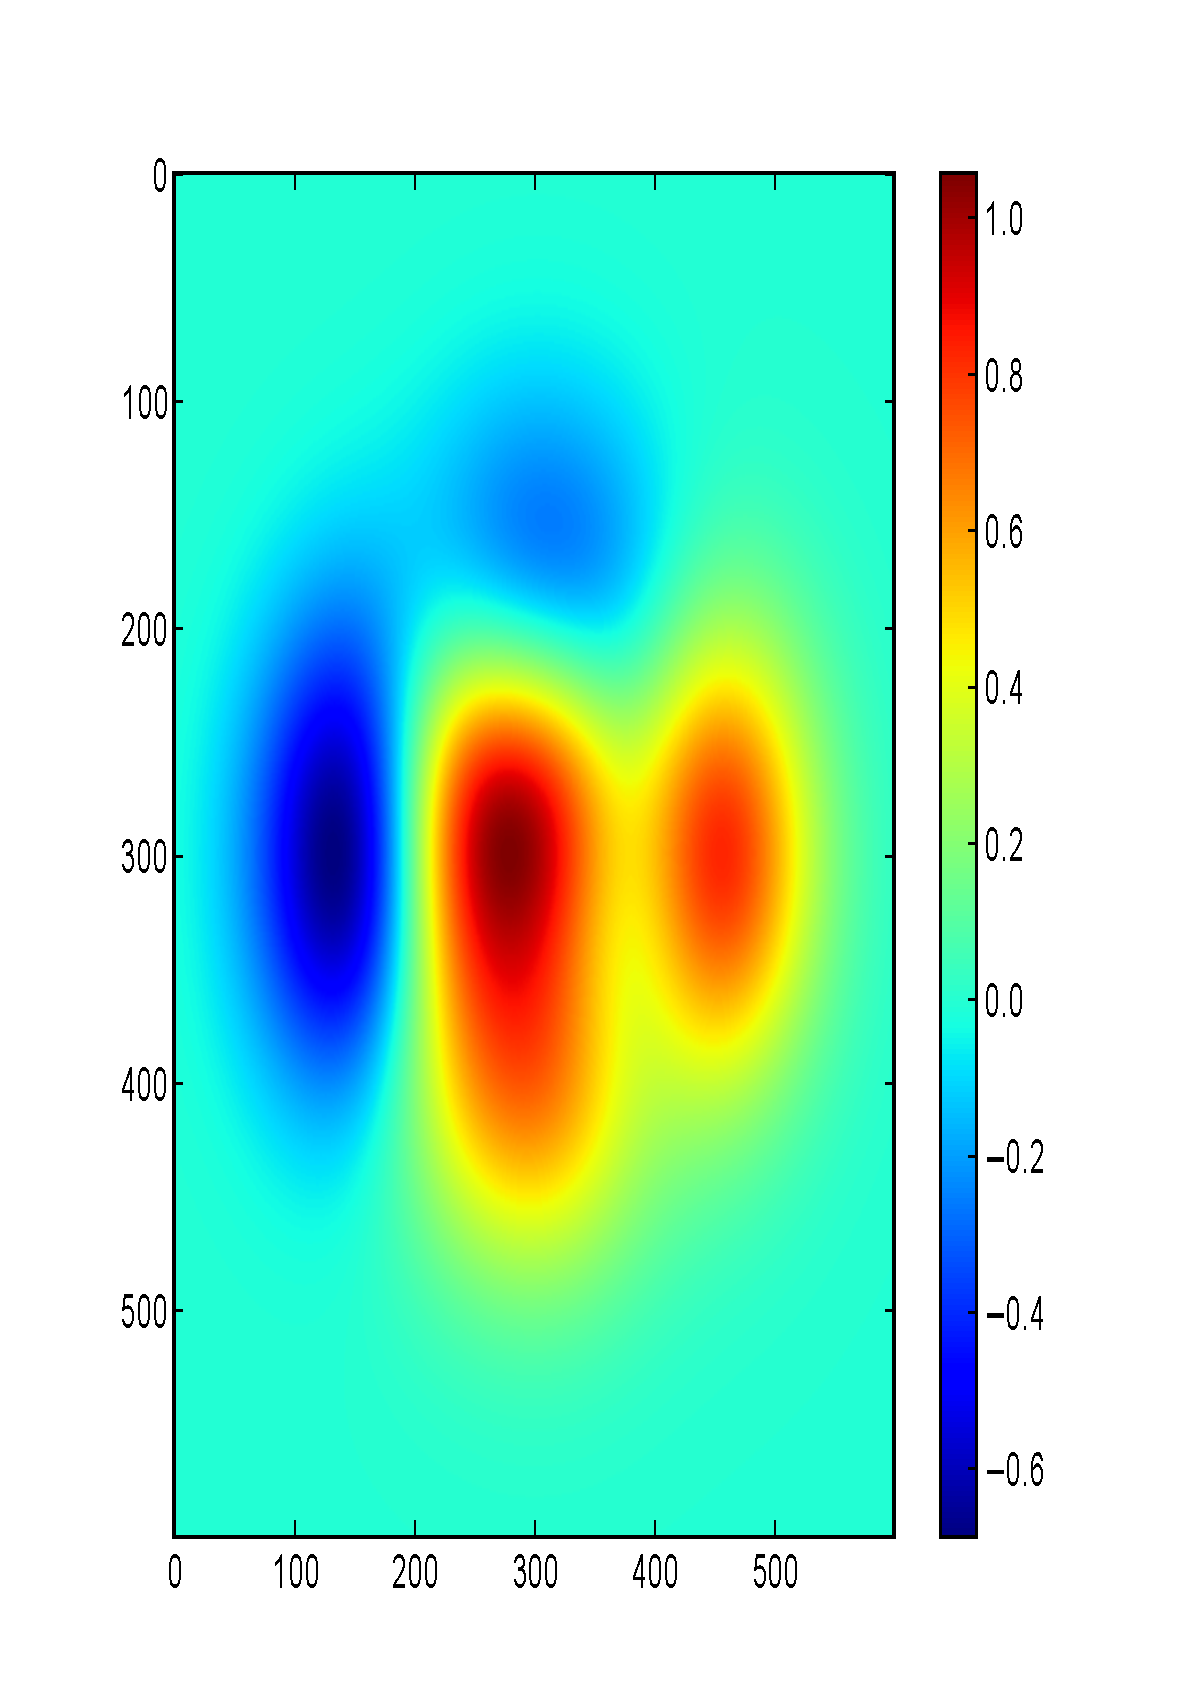
\includegraphics[height=\graphht]{Chapter-2/figs/color_stretched}
\caption{Here is a HUGE sample figure with a HUGE caption. Our goal is to make 
  a caption that is so long that the caption spills into the lower margin, 
  leading to an ETD error. The way to solve this problem in a systematic way is
  to calculate how many lines of text the caption will use, then adjust the size
  of the image, such that it leaves just enough space for your huge caption.
  How I am solving this problem is by providing a new variable called graphht 
  that stores how tall the image should be. Then, to calculate how tall to make 
  the figure, you use the new function that I am providing called
  calculategraphicstargetheight. This function has one argument. The argument
  of the function is how many lines of text you estimate that the caption
  occupies. You can always run your tex once, measure this number, and type it
  into the argument for the function. What the function will do (it is defined 
  in the preamble) is take into account the size you give it, the spacing of the
  chapter and the footer at the bottom, and then calculate the total vertical 
  space available. Thus, this function should be used for images that are taller
  than they are wide.}
\label{fig:longcap}
\end{figure}
%
\begin{figure}[hbtp]
\centering
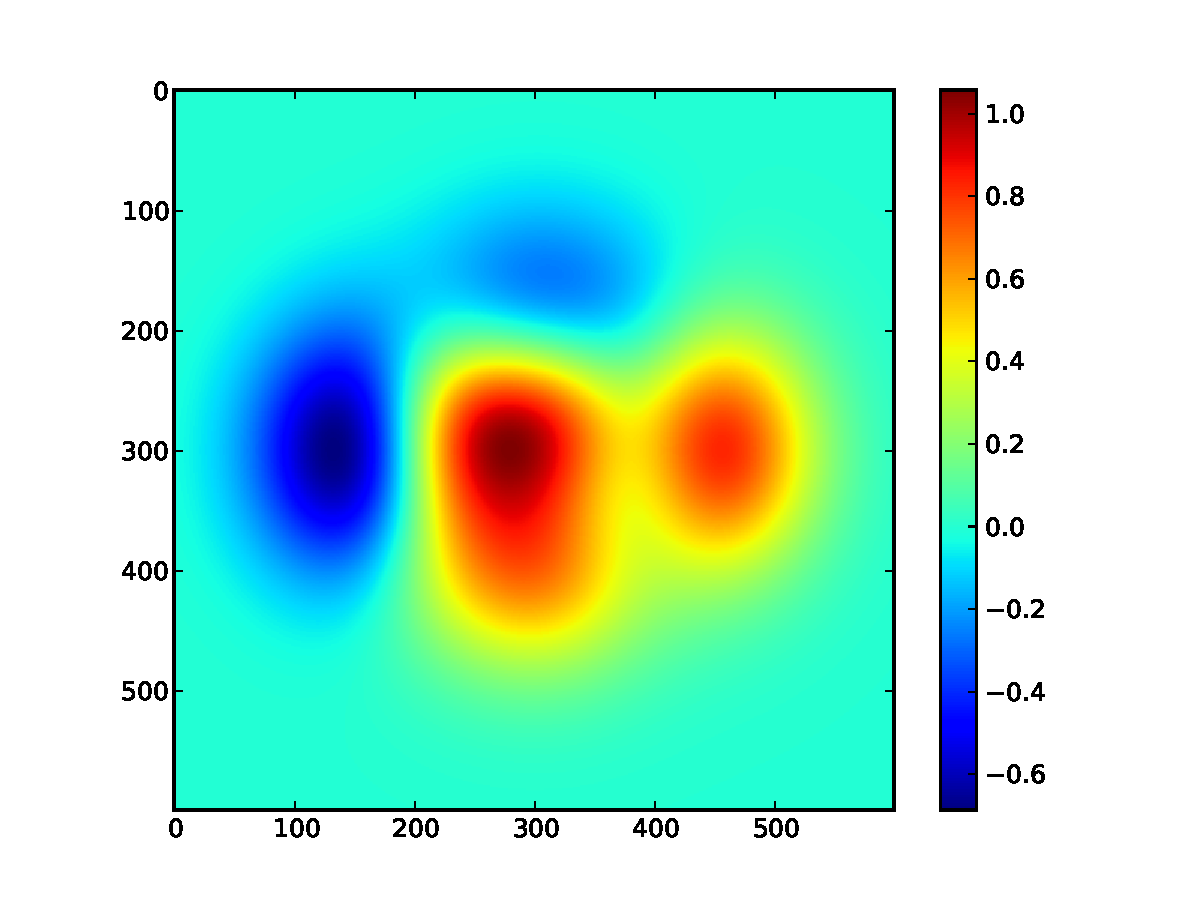
\includegraphics[width=0.6\textwidth]{Chapter-2/figs/color}
\caption{Here is a sample figure}
\label{fig:hist2}
\end{figure}
%
\begin{figure}[hbtp]
\centering
\subfloat[]{
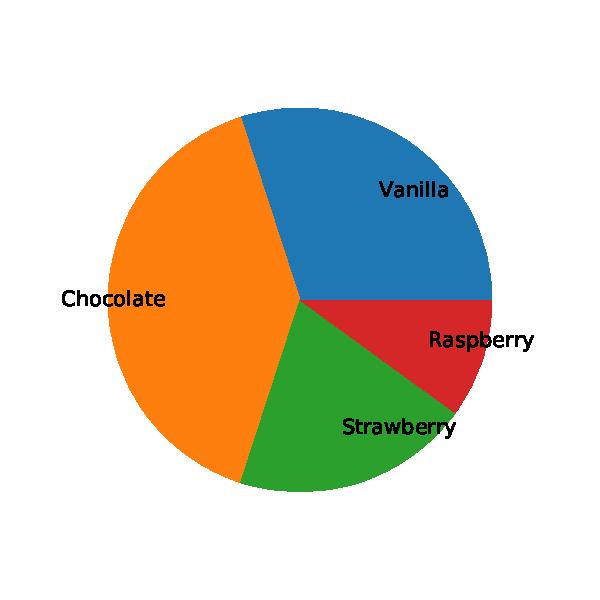
\includegraphics[width=0.4\textwidth]{Chapter-2/figs/pie}
}
\subfloat[]{
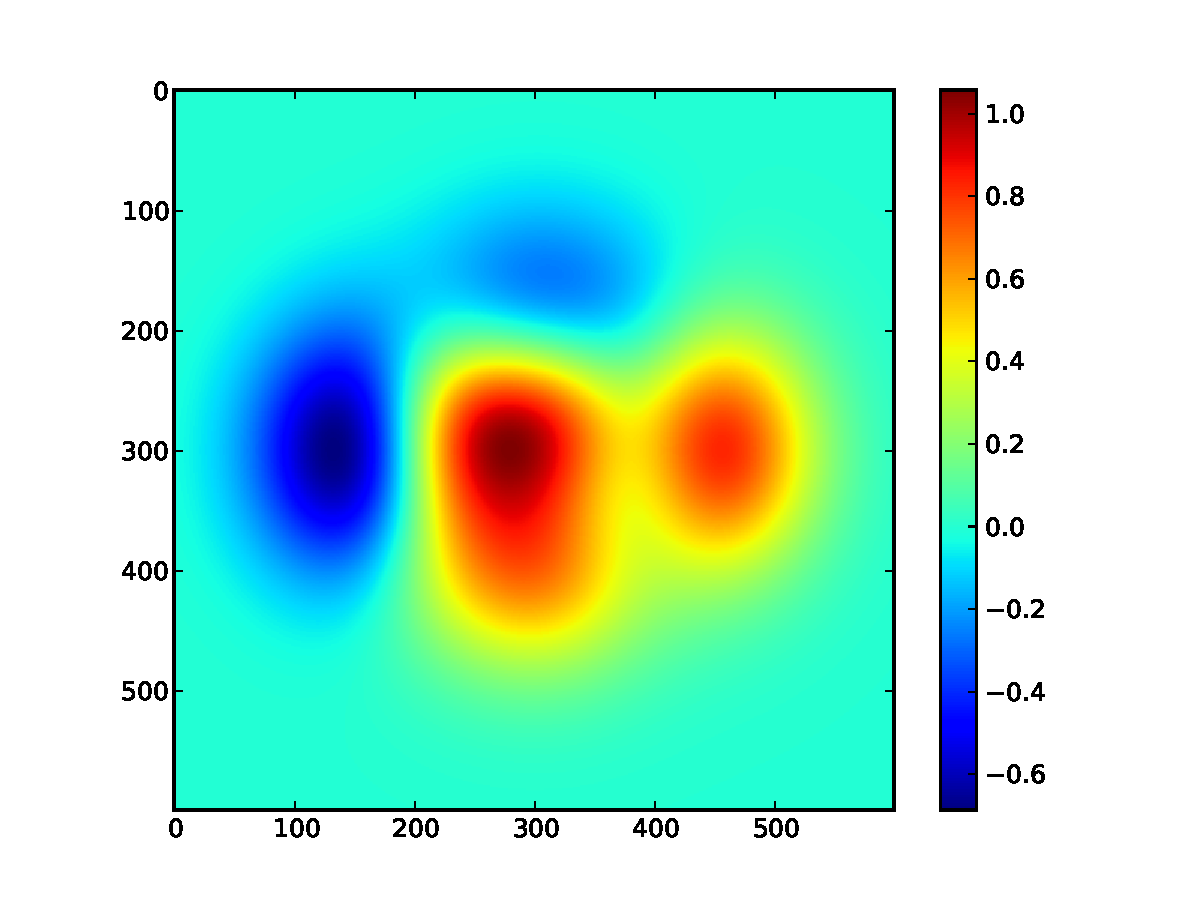
\includegraphics[width=0.4\textwidth]{Chapter-2/figs/color}
}
\caption{Here are two floating subfigures}
\label{fig:subfigures}
\end{figure}


\paragraph{Filler Text} \lipsum[12-15]

\newgeometry{margin=1in,lmargin=1.25in,footskip=\chapterfootskip, includehead, includefoot}
\thispagestyle{lscapedplain}
\begin{landscape}
\begin{figure}
\centering
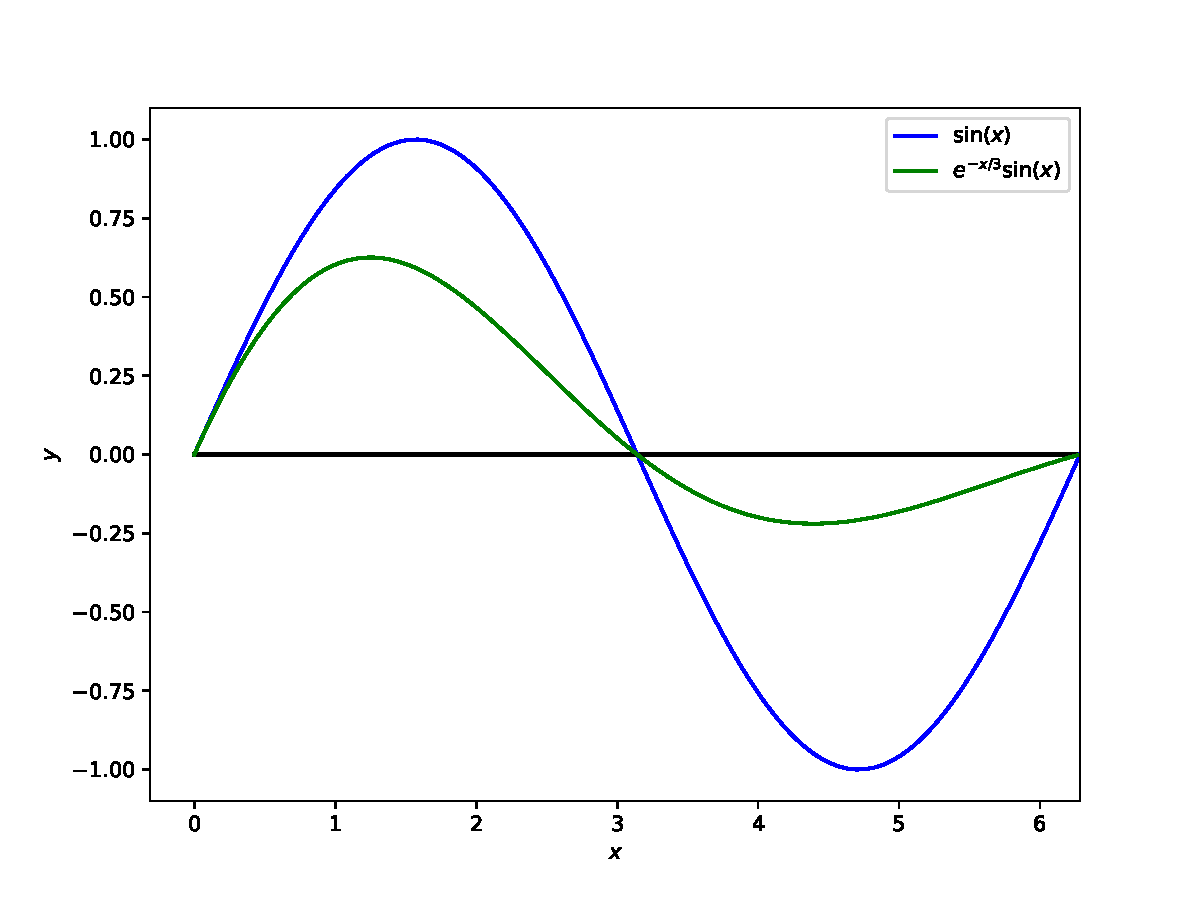
\includegraphics[width=\textwidth]{Chapter-2/figs/sine}
\caption{This figure has been turned sideways.  With large figures, 
         the author must ensure that there are at least two double spaces
         between the caption and the page number.}
\label{fig:hist}
\end{figure}
\end{landscape}
\restoregeometry
\pagestyle{plain}
\thispagestyle{plain}
\newgeometry{margin=1in,lmargin=1.25in,footskip=\chapterfootskip, includehead, includefoot}


\section{Matrices}
Let's look at a simple example of a matrix:
\[ \left( \begin{array}{ccc}
a & b & c \\
d & e & f \\
g & h & i \end{array} \right)\] 
%
You may prefer to write it this way:
\[ \left[\begin{array} {cccccc}
1 & 0 & 0 & 0 & 0 & 0 \\
0 & 1 & 0 & 0 & 0 & 0 \\
0 & 0 & 1 & 0 & 0 & 0 \\
0 & 0 & 0 & 1 & 0 & 0 \\
0 & 0 & 0 & 0 & 1 & 0 \\
0 & 0 & 0 & 0 & 0 & 1 \\
\end{array} \right] \]

\chapter{LOREM IPSUM}

\section*{A First Section}

\paragraph{Filler Text} \lipsum[1-6]
%
\begin{figure}[t]
  \centering
  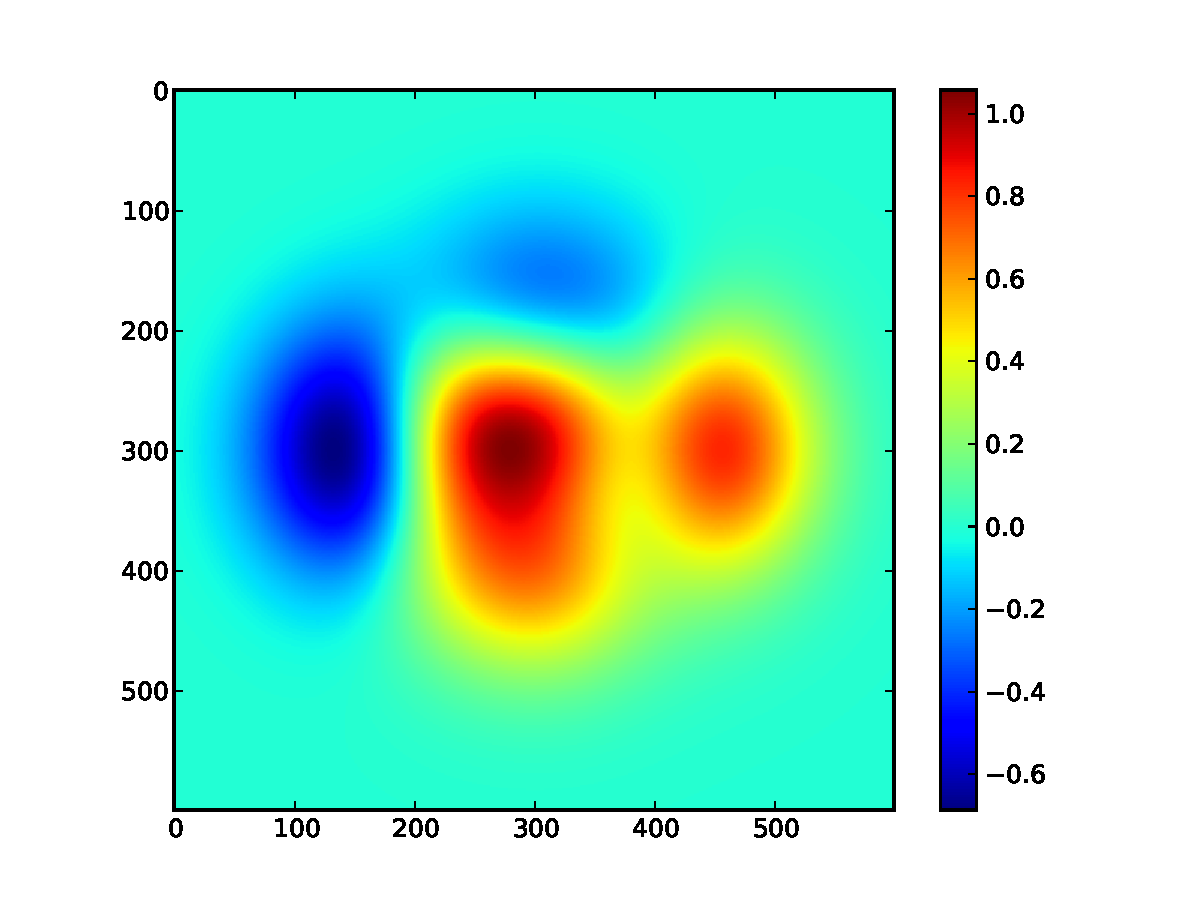
\includegraphics[width=0.6\textwidth]{Chapter-2/figs/color}
  \caption{A figure at the top of the page.}
  \label{fig:ch3.1}
\end{figure}
%
\lipsum[7-13]
%
\begin{figure}[!h]
  \centering
  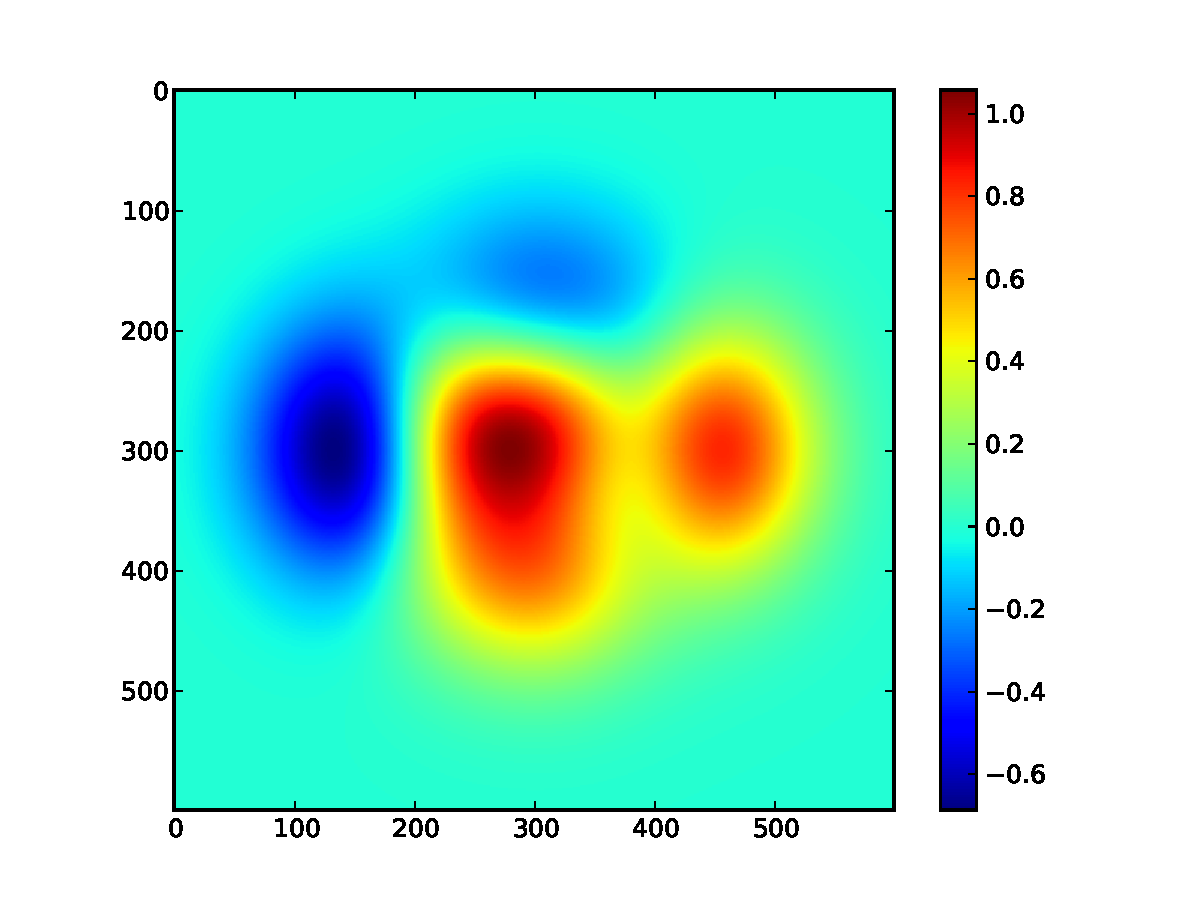
\includegraphics[width=0.6\textwidth]{Chapter-2/figs/color}
  \caption{A figure in the middle of text.}
  \label{fig:ch3.2}
\end{figure}
%
\begin{figure}[!b]
  \centering
  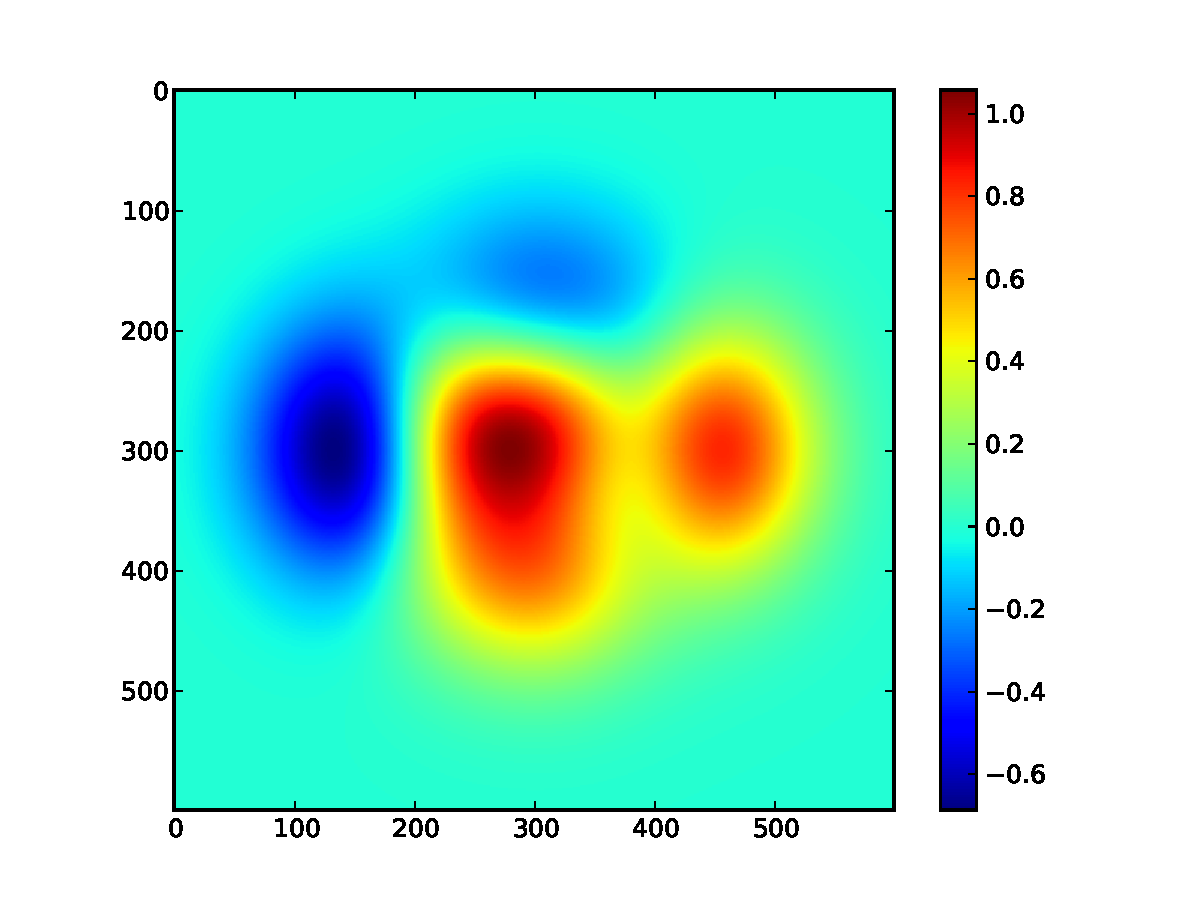
\includegraphics[width=0.6\textwidth]{Chapter-2/figs/color}
  \caption{A figure at the bottom of the page.}
  \label{fig:ch3.3}
\end{figure}
%
\lipsum[14-20]

%\include{Chapter-4/Chapter-4}
%\include{Chapter-5/Chapter-5}
%\include{Chapter-6/Chapter-6}
%\restoregeometry


%%---------------------------------------------------------------------------%%
%%  Bibliography 
%\ensureoddstart
\begin{spacing}{1}
 \setlength\bibitemsep{11pt} %22pt = 2*11pt, where fontsize is 11pt
 \phantomsection
 %\textorpdfstring and \uppercase needed due to hyperref package 
 % http://www.latex-community.org/forum/viewtopic.php?f=44&t=16601
 \addcontentsline{toc}{chapter}{\bibname}
 %\vspace{-0.5in}
\titleformat{\chapter}[display]{\bf\filcenter
}{\chaptertitlename\ \thechapter}{11pt}{\bf\filcenter}
\titlespacing*{\chapter}{0pt}{-0.5in-9pt}{22pt}

\printbibliography[heading=myheading]
\end{spacing}
%\bibliographystyle{apalike}

%%---------------------------------------------------------------------------%%
% Appendices
%\ensureoddstart
\restoregeometry
\appendix
\newgeometry{margin=1in,lmargin=1.25in,footskip=\chapterfootskip, includehead,
  includefoot}

\chapter{LOREM IPSUM}

\section{A First Section}

\paragraph{Filler Text} \lipsum[1-6]
%
\begin{figure}
  \centering
  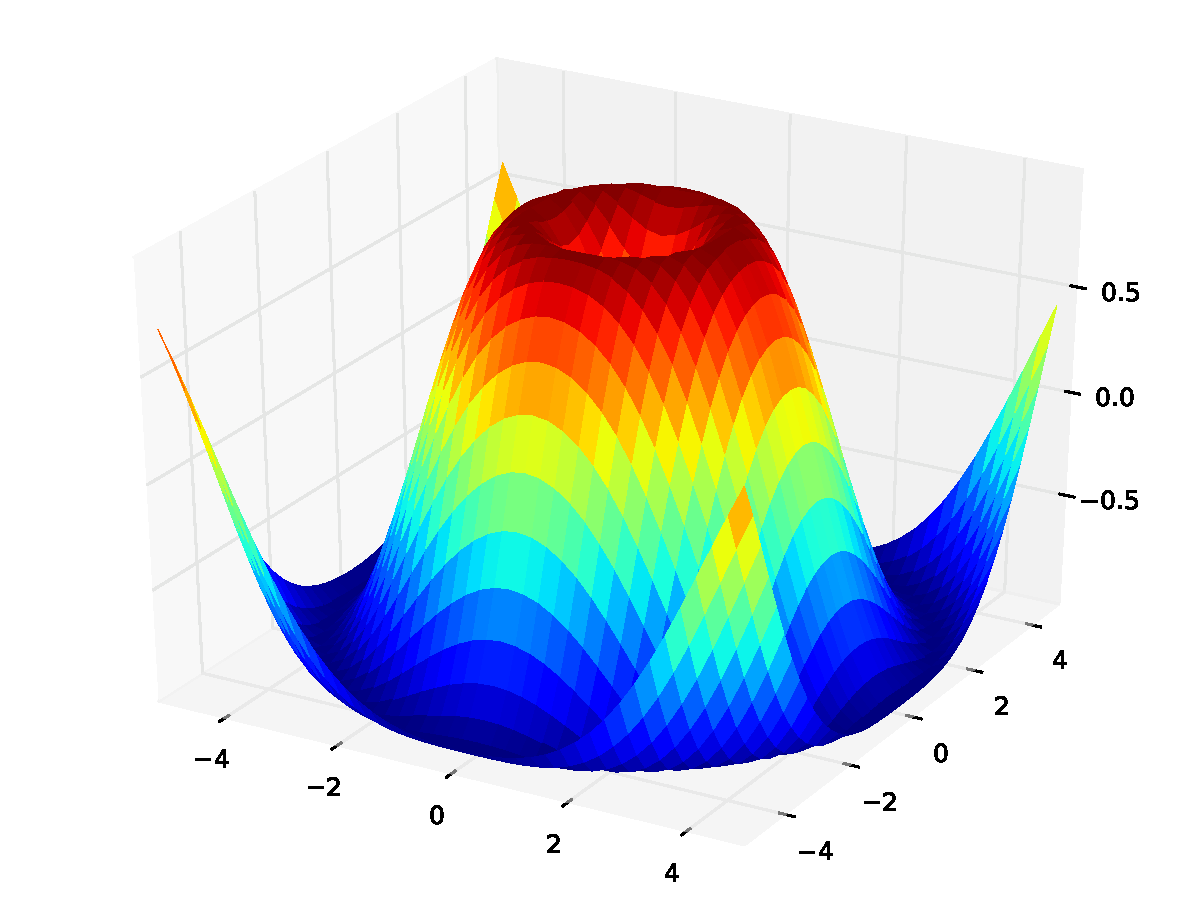
\includegraphics[width=0.6\textwidth]{Chapter-2/figs/threed}
  \caption{A figure in the appendix.}
  \label{fig:app}
\end{figure}
%
\lipsum[7-10]
\begin{table}
  \caption{A table in the appendix.}
  \label{tab:app}
  \begin{center}
    \begin{tabular}{lc}
      \toprule
      System & Author \\
      \midrule
      \TeX   & Donald Knuth   \\
      \LaTeX & Leslie Lamport \\
      \bottomrule
    \end{tabular}
  \end{center}
\end{table}
%

\section{A Second Section}

\lipsum[14-15]


\restoregeometry

%%---------------------------------------------------------------------------%%
%\ensureoddstart
\backmatter

\end{document}
